\documentclass[a4paper]{article}

%% Language and font encodings
\usepackage[english]{babel}
\usepackage[utf8x]{inputenc}
\usepackage[T1]{fontenc}

%% Sets page size and margins
\usepackage[a4paper,top=3cm,bottom=2cm,left=3cm,right=3cm,marginparwidth=1.75cm]{geometry}

%% Useful packages

\usepackage{graphicx}
\usepackage[colorinlistoftodos]{todonotes}
\usepackage[colorlinks=true, allcolors=blue]{hyperref}
\usepackage{cite}

\title{IF685 - Gerenciamento de Dados e Informação}
\author{Luan Advincula}

\begin{document}
\maketitle


\section{Introdução}

A disciplina de Gerenciamento de Dados e Informação tem por objetivo fornecer aos alunos uma base sólida em banco de dados, abrangendo desde conceitos de modelagem até recursos de linguagens de 4ª geração. Os projetos disciplinares da cadeira são baseados em tópicos de definição de minimundo, modelagem E-R, esquema relacional organizado, implementação relacional, SQL ("Structured Query Language", ou Linguagem de Consulta Estruturada), entre outros assuntos de computação.\cite{1} Outro ponto importante da disciplina é a modelagem de dados, que consiste na criação de um modelo físico que explique a lógica por traz do sistema, e com ele explicar as características de funcionamento e comportamento de um software.\cite{2} A disciplina se insere na área de Análise de Sistemas, justificada pelo ensino da dasciplina em relação a conceitos de banco de dados.\cite{3}  


\section{Relevância}

Levando em conta que essa disciplina tem um papel importante em uma das áreas mais influentes da computação (Análise de Dados), ela é muito importante para os alunos que se identificam com essa área específica ou têm vontade de trabalhar com a mesma.

\subsection{Pontos Importantes}
\begin{itemize}
\item Ela dá uma noção básica e aplicada de banco de dados.
\item É uma matéria que explica e exemplifica conceitos e informações que fazem diferença no mercado de trabalho.
\item Apresenta conceitos de Modelagem E-R, Linguagen da 4ª Geração, SQL, e XML (Extensible Markup Language).
\todo[inline]{O que é um Banco de Dados?\\ É um grupo de arquivos relacionados entre si, com informações sobre alguém, algo ou algum lugar.}

\end{itemize}



\section{Relação com outras disciplinas}
\begin{table}[h]
\centering
\label{my-label}
\begin{tabular}{|l|l|}
\hline
\begin{tabular}[c]{@{}l@{}}IF669 - Introdução a \\ Computação\end{tabular}         & \begin{tabular}[c]{@{}l@{}}Essa disciplina, como o nome já diz, introduz conceitos de \\ programação que serão essenciais para não só essa, mas \\ também para muitas outras disciplinas do curso.\end{tabular} \\ \hline
\begin{tabular}[c]{@{}l@{}}IF672 - Algoritmos e \\ Estrutura de Dados\end{tabular} & \begin{tabular}[c]{@{}l@{}}Essa disciplina introduz o conceito de dados, que será \\ amplamente usado na disciplina de Gerenciamento de \\ Dados e Informação.\end{tabular}                                  \\ \hline
\end{tabular}
\end{table}

\section{Referências Bibliográficas da Disciplina}
\begin{enumerate}
\item Elmasri e S. Navathe – Sistemas de Banco de Dados, Pearson Education, 2011, 6ª edição.
\item R. Ramakrishnam e J. Gehrke – Sistemas de Gerenciamento de Banco de Dados – McGraw Hill, 2008.
\item A. Silberschartz, H. Korth e S. Sudarshan – Sistemas de Banco de Dados, Makron Books, 2006, 4ª edição.
\item J. Price – Oracle Database 11g - SQL, Bookman, 2009.
\item R. Baeza-Yates e B. Ribeiro-Neto – Modern Information Retrieval, Addison Wesley, 1999.
\item K. Laudon e J. Laudon – Sistemas de Informações Gerenciais, Pearson Education, 2011, 9ª edição.
\end{enumerate}

\begin{figure}
\centering
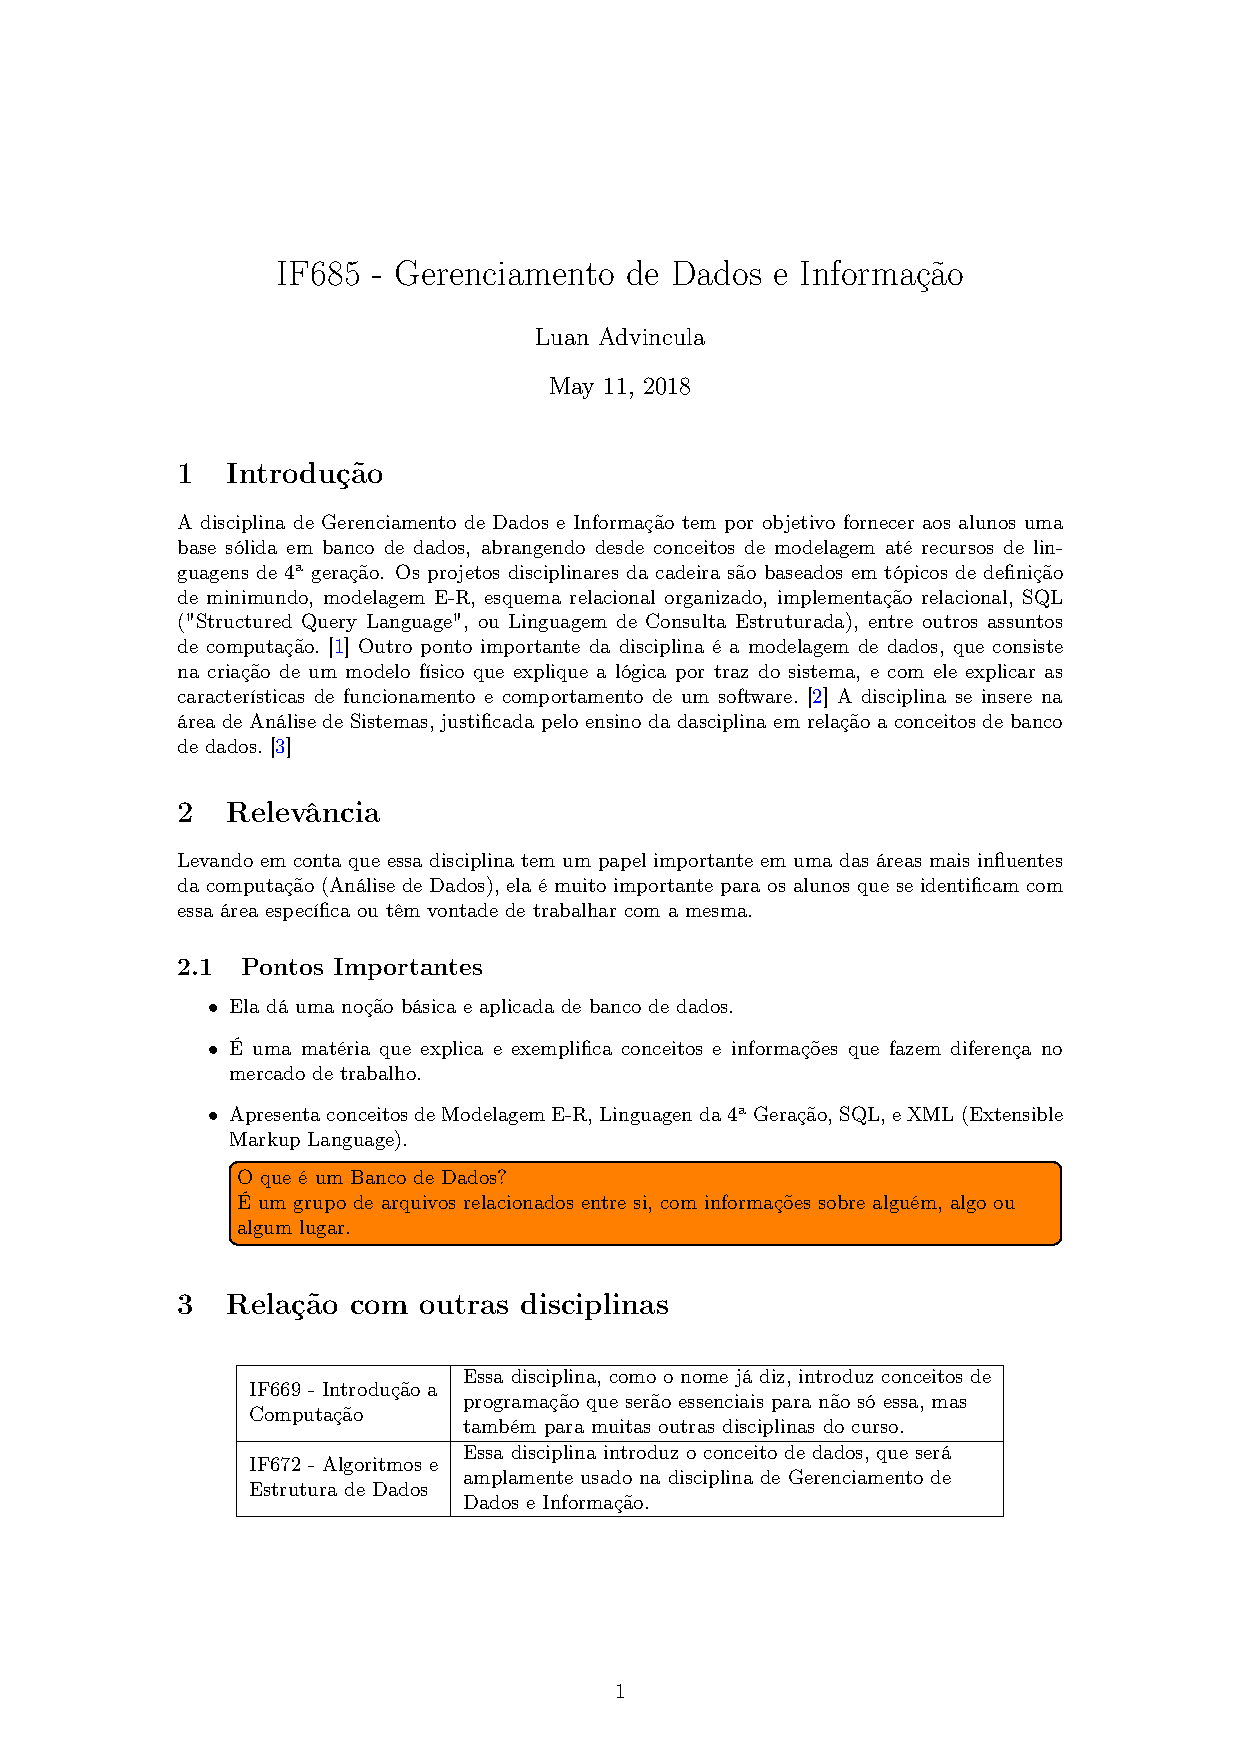
\includegraphics[width=0.3\textwidth]{lssa.jpg}
\caption{\label{fig:lssa}Representação de um Banco de Dados - CC0 1.0 Universal (CC0 1.0). }
\end{figure}


\bibliographystyle{unsrt}
\bibliography{lssa}


\end{document}